\documentclass
[handout]
{beamer}


%%
%%
%%
% From http://tex.stackexchange.com/questions/2072/beamer-navigation-circles-without-subsections
% Solution #2 or 3:
% \usepackage{etoolbox}
% \makeatletter
% % replace the subsection number test with a test that always returns true
% \patchcmd{\slideentry}{\ifnum#2>0}{\ifnum2>0}{}{\@error{unable to patch}}%
% \makeatother
% Solution #1:
\usepackage{remreset}% tiny package containing just the \@removefromreset command
\makeatletter
\@removefromreset{subsection}{section}
\makeatother
\setcounter{subsection}{1}


\usepackage{etex}
\usepackage{pgf}
\usepackage{tikz}
\usepackage{url}
\usepackage{amsmath}
\usepackage{color}
% \definecolor{red}{rgb}{1,0,0}
\usepackage{ulem}
% \usepackage{booktabs}
\usepackage{colortbl,booktabs}
\renewcommand*{\thefootnote}{\fnsymbol{footnote}}
\usepackage{fancybox}
\usepackage[framemethod=TikZ]{mdframed}
\mdfdefinestyle{FactStyle}{%
  outerlinewidth=0.5,
  roundcorner=1pt,
  leftmargin=1cm,
  linecolor=blue,
  outerlinecolor=blue!70!black,
  backgroundcolor=yellow!40
}
\usepackage{cancel}

  \newcommand\Warning{%
    \makebox[2.4em][c]{%
      \makebox[0pt][c]{\raisebox{.2em}{\Large!}}%
      \makebox[0pt][c]{\color{red}\Huge$\bigtriangleup$}}}%

\usepackage{stackengine}
\usepackage{scalerel}
\usepackage{xcolor}
  \newcommand\dangersign[1][2ex]{%
    \renewcommand\stacktype{L}%
    \scaleto{\stackon[1.3pt]{\color{red}$\triangle$}{\tiny !}}{#1}%
  }



\usepackage{dcolumn}
\newcolumntype{d}[1]{D{.}{.}{#1}}

% From
% http://tex.stackexchange.com/questions/109900/how-can-i-box-multiple-aligned-equations
\usepackage{empheq}
\usepackage{tcolorbox}  \newtcbox{\othermathbox}[1][]{%
  nobeforeafter, tcbox raise base, 
  colback=black!10, colframe=red!30, 
  left=1em, top=0.5em, right=1em, bottom=0.5em}

\newcommand\blue{\color{blue}}
\newcommand\red{\color{red}}
\newcommand\green{\color{green!75!black}}
\newcommand\purple{\color{purple}}
\newcommand\bluegreen{\color{blue!75!green}}
\newcommand\orange{\color{orange}}
\newcommand\redgreen{\color{red!50!green}}
\newcommand\grey{\color{black}}
\newcommand\gap{\vspace{.1in}}
\newcommand\nb{${\red\bullet}\ $}
\newcommand\halfgap{\vspace{.05in}}
\newcommand\divideline{\line(1,0){352}}
\usepackage{marvosym} % for \Smiley

\newcommand{\bluealert}[1]{{\blue\textbf{#1}}}

% \usepackage{beamerthemesplit} %Key package for beamer
\usetheme{Singapore}
% \usetheme{Szeged}
% \usetheme{Garfield}
% \usetheme{CambridgeUS}
% \usenavigationsymbolstemplate{} %Gets rid of slide navigation symbols


\setbeamercolor{separation line}{use=structure,bg=structure.fg!50!bg}
% \begin{beamercolorbox}[colsep=0.5pt]
%   {upper separation line foot}
% \end{beamercolorbox}



\makeatletter
\setbeamertemplate{footline}
{
  \leavevmode%
  \hbox{%
% \begin{beamercolorbox}[colsep=0.5pt]
%   {upper separation line foot}
% \end{beamercolorbox}


  \begin{beamercolorbox}[wd=.5\paperwidth,ht=2.25ex,dp=2ex,colsep=0.5pt]%
    {upper separation line foot}
    \usebeamerfont{author in head/foot}%
    \hspace*{2ex}\insertshortdate:\ \insertshorttitle
  \end{beamercolorbox}%
  \begin{beamercolorbox}[wd=.5\paperwidth,ht=2.25ex,dp=2ex,right]{title in head/foot}%
    \usebeamerfont{title in head/foot}
    {\insertshortauthor}\hspace*{2ex}
  \end{beamercolorbox}}%
  % \begin{beamercolorbox}[wd=.333333\paperwidth,ht=2.25ex,dp=2ex,right]{date in head/foot}%
  %   \usebeamerfont{date in head/foot}\insertshortdate{}\hspace*{2em}
  %   \insertframenumber{} / \inserttotalframenumber\hspace*{2ex} 
  % \end{beamercolorbox}%
  \vskip0pt%
}
\makeatother

\usetikzlibrary{decorations.markings}
\usetikzlibrary{arrows}


\title{Final Exam Review}
\author{Peter Garfield, UCSB Mathematics}
\date{March 15, 2017}
%\institute{}


\useinnertheme{default}

\usefonttheme{serif}
% \usecolortheme{rose}
% \usecolortheme{whale}
% \usecolortheme{orchid}
\usecolortheme{crane}
% \usecolortheme{dolphin}


%TEMPLATE
\setbeamertemplate{navigation symbols}{}

\setbeamertemplate{note page}[compress]

\setbeamertemplate{frametitle}{
  \vspace{0.5em}
  % \begin{centering}
  {\huge\blue\textbf{\textmd{\insertframetitle}}}
  \par
  % \end{centering}
}

% From http://tex.stackexchange.com/questions/7032/good-way-to-make-textcircled-numbers:
\newcommand*\circled[1]{\tikz[baseline=(char.base)]{\node[shape=circle,draw,fill=orange,inner sep=1pt] (char) {#1};}} 
% \renewcommand{\labelenumi}{\circled{\textbf{\arabic{enumi}}}}

\let\olddescription\description
\let\oldenddescription\enddescription
\usepackage{enumitem}
\let\description\olddescription
\let\enddescription\oldenddescription

% \usepackage[loadonly]{enumitem}
\setlist[enumerate,1]{label=\colorbox{orange}{\arabic*.},font=\bfseries}
%\setlist[enumerate,2]{label=\colorbox{blue!25}{(\alph*)},font=\bfseries}
% \setlist[enumerate,1]{label=\arabic*.,font=\bfseries}
\setlist[itemize,1]{label=\red$\bullet$}
\setlist[itemize,2]{label=\blue$\bullet$}

\newcommand\answer[1]{\fbox{#1}}
% \renewcommand\answer[1]{}

\newcommand{\antilog}{\operatorname{antilog}}








\title{final review}
\author{Trevor Klar, UCSB Mathematics}
\date{July 25, 2022}



\begin{document}
\small
\renewcommand{\fbox}{}



\frame{
  \frametitle{}
  {\Huge{}Welcome To Math 34A!}\\[.5em]

  {\Huge{}Differential Calculus}
  \vfill
  {\Large{}Instructor:}\\
  \ \hspace*{0.2in} Trevor Klar, \url{trevorklar@math.ucsb.edu}\\
  \ \hspace*{0.2in} South Hall 6431X (Grad Tower, 6th floor, blue side, first door on the right)
  \\[0.5em]

  {\Large{}Office Hours:}\\
  \ \hspace*{0.2in} MTWR after class 2:00-3:00, and by appointment. Details on Gauchospace. 
  \bigskip

  {\tiny \copyright\ 2017-22\ Daryl Cooper, Peter Garfield, Ebrahim Ebrahim, Nathan Schley, and Trevor Klar}\\
  Please do not distribute outside of this course.
  \vfill

}


\section*{Videos}

\frame{
  \frametitle{Videos}

  {\blue Vsauce: Logarithmic thinking:} \vspace{4pt} \\  
   {\blue \url{https://www.youtube.com/watch?v=Pxb5lSPLy9c&t=1m53s}} \vspace{.4in} \\ 
  {\blue 3Blue1Brown: Modeling Caronavirus Spread} \vspace{4pt} \\  {\blue \url{https://youtu.be/Kas0tIxDvrg}} \vspace{.4in} \\ 
  

}

\section*{Exam Topics}

\frame{
  \frametitle{Final Exam: Wednesday, July 17, 12:30-1:35PM}

  {\Large\color{blue}Bring:}
  \begin{itemize}
  \item A pen or \alert{sharp} pencil.
  \item $3"\times5"$ cards with your notes. {\bf Three} notecards allowed. \pause \\ 
  {\blue This is not a typo. The exam is 3 hours long.} \pause
  \item Student ID.
  \end{itemize}
  \bigskip

  {\Large\color{red}Don't bring:}
  \begin{itemize}
  \item A calculator
  \end{itemize}
  \smallskip

  Please Be Early! 

    Exam is cumulative, with its focus spread to all topics. 
    
    {\bf Please study the topics beyond just formulas and procedures.} This approach will set you up the for success. 

}



\frame{
  \frametitle{Final Exam: Wednesday, July 17, 12:30-1:35PM}

Here are the topics we've covered:
\begin{itemize}
\item\pause
percentages, inverse functions, pythagorean theorem, units, areas and volumes, and lines.
\item\pause
general topics from ch1 like word problems, substitution, and solving equations.
\item\pause
limits, sums, change in a function, percent error, exponentiation, logarithms
\item\pause
related types of word problems: like half-life and doubling time, etc.
\item\pause
calculus! (i.e. derivatives)
\end{itemize}
}
\frame{
Here's a more detailed list of topics relating to derivatives:
\begin{itemize}
\item\pause
calculus! (i.e. derivatives)
\begin{itemize}
\item\pause
  finding derivatives of expressions (mostly things made out of $x^n$ and $e^{kx}$)
\item\pause
  understanding the definition of derivative (limit of average rate of change/slope of secant line)
\item\pause
  linear approximation (finding and using eqn of tangent line, or just using derivative to get useful info somehow)
\item\pause
  second derivative and concavity
\item\pause
  optimization and the related word problems
\end{itemize}
\end{itemize}
}


\frame{
  \frametitle{Grade Breakdown}

Homework 20\% \vspace{15pt} \\
Quizzes 10\% \vspace{15pt} \\
Midterm Exams 40\% (Worth 20\% each) \vspace{15pt} \\
Final Exam 30\% \vspace{15pt} \\

\pause

iclicker - up to 3\% extra credit  \vspace{15pt} \\

\pause

%{\blue If your \underline{in-class} final score is higher than the grade you would get in the class according to the rubric above, and assuming you have no suspicious answers on any quizzes or exams (which is the vast majority of you!), then your grade will be based entirely on that score.} \vspace{15pt} \\




}


\section*{Review of Recent things}

\frame{
\centerline{\Huge \blue Let's refresh} \vspace{20pt} 

\centerline{\Huge \blue some Calculus}

}

\frame{
The derivative of $y$ with respect to $x$ tells us the rate of change, \pause {\blue but it depends on the current value of $x$!} \pause

\vspace{1em}

If we write $y$ as a function of $x$ like this: $y=f(x)$, then the derivative is written as
$$
\begin{array}{ccccc}
\dfrac{\textrm{d}y}{\textrm{d}x} & \text{or} & \dfrac{\textrm{d}f}{\textrm{d}x} & \text{or} & f'(x)
\end{array}
$$
\pause
It is the limit of ``average rate of change'' over shorter and shorter $\Delta x$:
$$ f'(x) = \lim_{h \rightarrow 0} \frac{f(x+h)-f(x)}{h} $$
also known as ``instantaneous rate of change''
}


\frame{
  \frametitle{Differentiation Power Moves}

  \begin{minipage}[b]{0.35\linewidth}
    \begin{empheq}[box=\othermathbox]{align*}
      \frac{d}{dx}\left(e^{{\red k}x}\right)
      & = {\red k}e^{{\red k}x}
    \end{empheq}
  \end{minipage}
  \hspace*{0.2in}
  \pause 
  and
  \hspace*{0.2in}
  \begin{minipage}[b]{0.35\linewidth}
    \begin{empheq}[box=\othermathbox]{align*}
      \frac{d}{dx}\left(x^{{\red n}}\right)
      & = {\red n} x^{{\red n}-1}
    \end{empheq}
  \end{minipage}
  \bigskip



  \alert{Question:}\ Find $\dfrac{d}{dx}\left( 3x^2 + 4e^{-2x} - x^3\right)$
  \begin{center}
    A$=12e^{2x}+15x^2$
    \qquad
    B$ = 12e^{3x}+15 x^3$
    \qquad
    C$ = 4e^{3x}+15x^2$
    \\
    \
    \quad
    D$=6x + 8e^{-2x} - 15x^2$
    \quad
    E$= \text{Other}$
    \pause
    \quad
    \fbox{E}
  \end{center}

}


\frame{
  \frametitle{Tangent Line Approximation}

  To do a tangent line approximation:
  \begin{itemize}
  \item[(i)] Find the equation of the tangent line.

  \item[(ii)] Plug in the required value(s) into this equation.

  \end{itemize}
}


\frame{
  \frametitle{Meanings: The First Derivative}

  \begin{center}
    \begin{tikzpicture}[x=15mm,y=5mm,>=latex]
      \only<1>{%
        \draw[ultra thick,blue,domain=-1:3,smooth] plot (\x,{(\x)^3-3*(\x)^2+2});
      }
      \only<2->{%
        \draw[ultra thick,blue,domain=-1:0,smooth] plot (\x,{(\x)^3-3*(\x)^2+2});
        \draw[ultra thick,red,domain=0:2,smooth] plot (\x,{(\x)^3-3*(\x)^2+2});
        \draw[ultra thick,blue,domain=2:3,smooth] plot (\x,{(\x)^3-3*(\x)^2+2});
        \filldraw[green] (0,2) circle (2pt);
        \filldraw[green] (2,-2) circle (2pt);
      }
      \uncover<3->{%
        \draw[ultra thick,blue,<-] (-1,-2.5) -- (0,-2.5);
        \draw[blue,fill=white] (0,-2.5) circle (2pt);
        \draw[ultra thick,blue,->] (2,-2.5) -- (3,-2.5);
        \draw[blue,fill=white] (2,-2.5) circle (2pt);
        \draw[ultra thick,red] (0,-2.85) -- (2,-2.85);
        \draw[red,fill=white] (0,-2.85) circle (2pt);
        \draw[red,fill=white] (2,-2.85) circle (2pt);
        \node[blue] at (-0.5,-3.5) {$f(x)$ incr};
        \node[red] at (1,-3.5) {$f(x)$\ decr};
        \node[blue] at (2.5,-3.5) {$f(x)$\ incr};
      }
      \uncover<5->{%
        \node[blue] at (-0.5,-4.5) {$f'(x)>0$};
        \node[red] at (1,-4.5) {$f'(x)<0$};
        \node[blue] at (2.5,-4.5) {$f'(x)>0$};
      }
      \begin{scope}
        \clip (-1.5,-4) rectangle (3.5,2.75);
              \uncover<4->{%
        \draw[thick,blue,domain=-1:0] plot (\x,{(-1/2)^3-3*(-1/2)^2+2+3*(-1/2)*(-1/2-2)*(\x+1/2)});
        \draw[thick,red,domain=0:1.85] plot (\x,{(1)^3-3*(1)^2+2+3*(1)*(1-2)*(\x-1)});
        \draw[thick,blue,domain=2.2:3.5] plot (\x,{(2.5)^3-3*(2.5)^2+2+3*(2.5)*(2.5-2)*(\x-2.5)});
        \fill[black] (-0.5,{(-1/2)^3-3*(-1/2)^2+2}) circle (2pt);
        \fill[black] (1,{(1)^3-3*(1)^2+2}) circle (2pt);
        \fill[black] (2.5,{(2.5)^3-3*(2.5)^2+2}) circle (2pt);
      }
      \end{scope}
    \end{tikzpicture}
  \end{center}
  \bigskip

  \uncover<6->{%
    \bluealert{Point:}

    \begin{mdframed}[style=FactStyle]
      \vspace*{-1.25em}
      \begin{align*}
        {\blue f'(x) > 0} & \iff\ \text{$f(x)$\ is increasing} \\
        {\red f'(x) < 0} & \iff\ \text{$f(x)$\ is decreasing}
      \end{align*}
    \end{mdframed}
  }
  \vspace*{3in}

}


\frame{
  \frametitle{Meanings: The Second Derivative}

  \begin{center}
    \begin{tikzpicture}[x=15mm,y=5mm,>=latex]
      \only<1>{%
        \draw[ultra thick,blue,domain=-1:3,smooth] plot (\x,{(\x)^3-3*(\x)^2+2});
      }
      \only<2->{%
        \draw[ultra thick,green!50!black,domain=-1:1,smooth] plot (\x,{(\x)^3-3*(\x)^2+2});
        \draw[ultra thick,orange!90!black,domain=1:3,smooth] plot (\x,{(\x)^3-3*(\x)^2+2});
        \filldraw[blue] (1,0) circle (2pt);
      }
      \uncover<3->{%
        \draw[ultra thick,green!50!black,<-] (-1,-2.5) -- (1,-2.5);
        \draw[green!50!black,fill=white] (1,-2.5) circle (2pt);
        \draw[ultra thick,orange!90!black,->] (1,-2.85) -- (3,-2.85);
        \draw[orange!90!black,fill=white] (1,-2.85) circle (2pt);
        \node[green!50!black] at (0,-3.5) {$f(x)$ cc down};
        \node[orange!90!black] at (2,-3.5) {$f(x)$\ cc up};
      }
      \begin{scope}
        \clip (-1.5,-4) rectangle (3.5,2.75);
              \uncover<4->{%
        % Tangent lines to $y=x^3-3x^2+2$ has slope $y'=3x^2-6x=3x(x-2)$.
        % \draw[blue,domain=-1:0] plot (\x,{(-5/5)^3-3*(-5/5)^2+2+3*(-5/5)*(-5/5-2)*(\x+5/5)});
        % \draw[blue,domain=-1:0] plot (\x,{(-4/5)^3-3*(-4/5)^2+2+3*(-4/5)*(-4/5-2)*(\x+4/5)});
        % \draw[blue,domain=-1:0] plot (\x,{(-3/5)^3-3*(-3/5)^2+2+3*(-3/5)*(-3/5-2)*(\x+3/5)});
        % \draw[blue,domain=-1:0] plot (\x,{(-2/5)^3-3*(-1/5)^2+2+3*(-2/5)*(-2/5-2)*(\x+2/5)});
        % \draw[blue,domain=-1:0] plot (\x,{(-1/5)^3-3*(-1/5)^2+2+3*(-2/5)*(-1/5-2)*(\x+1/5)});
        % \draw[blue,domain=-1:0] plot (\x,{(-1/3)^3-3*(-1/3)^2+2+3*(-1/3)*(-1/3-2)*(\x+1/3)});
        \draw[thick,green!50!black,domain=-1:0] plot (\x,{(-2/3)^3-3*(-2/3)^2+2+3*(-2/3)*(-2/3-2)*(\x+2/3)});
        \draw[thick,green!50!black,domain=-1:0.3333] plot (\x,{(-1/3)^3-3*(-1/3)^2+2+3*(-1/3)*(-1/3-2)*(\x+1/3)});
        \draw[thick,green!50!black] (-0.5,2) -- (0.5,2);
        \draw[thick,green!50!black,domain=-0.3333:1] plot (\x,{(1/3)^3-3*(1/3)^2+2+3*(1/3)*(1/3-2)*(\x-1/3)});
        \draw[thick,green!50!black,domain=0:1] plot (\x,{(2/3)^3-3*(2/3)^2+2+3*(2/3)*(2/3-2)*(\x-2/3)});
        % \draw[thick,red,domain=0:1.85] plot (\x,{(1)^3-3*(1)^2+2+3*(1)*(1-2)*(\x-1)});
        % \draw[thick,blue,domain=2.2:3.5] plot (\x,{(2.5)^3-3*(2.5)^2+2+3*(2.5)*(2.5-2)*(\x-2.5)});
        \fill[black] ({-2/3},{(-2/3)^3-3*(-2/3)^2+2}) circle (2pt);
        \fill[black] ({-1/3},{(-1/3)^3-3*(-1/3)^2+2}) circle (2pt);
        \fill[black] (0,2) circle (2pt);
        \fill[black] ({1/3},{(1/3)^3-3*(1/3)^2+2}) circle (2pt);
        \fill[black] ({2/3},{(2/3)^3-3*(2/3)^2+2}) circle (2pt);
        % \fill[black] (1,{(1)^3-3*(1)^2+2}) circle (2pt);
        % \fill[black] (2.5,{(2.5)^3-3*(2.5)^2+2}) circle (2pt);
      }
      \uncover<6->{%
        \draw[thick,orange!90!black,domain=2.3:3.3] plot (\x,{(8/3)^3-3*(8/3)^2+2+3*(8/3)*(8/3-2)*(\x-8/3)});
        \draw[thick,orange!90!black,domain=1.9:2.9] plot (\x,{(7/3)^3-3*(7/3)^2+2+3*(7/3)*(7/3-2)*(\x-7/3)});
        \draw[thick,orange!90!black] (1.5,-2) -- (2.5,-2);
        \draw[thick,orange!90!black,domain=1.3333:2.1] plot (\x,{(5/3)^3-3*(5/3)^2+2+3*(5/3)*(5/3-2)*(\x-5/3)});
        \draw[thick,orange!90!black,domain=0.5:2] plot (\x,{(4/3)^3-3*(4/3)^2+2+3*(4/3)*(4/3-2)*(\x-4/3)});
        % \draw[thick,red,domain=0:1.85] plot (\x,{(1)^3-3*(1)^2+2+3*(1)*(1-2)*(\x-1)});
        % \draw[thick,blue,domain=2.2:3.5] plot (\x,{(2.5)^3-3*(2.5)^2+2+3*(2.5)*(2.5-2)*(\x-2.5)});
        \fill[black] ({4/3},{(4/3)^3-3*(4/3)^2+2}) circle (2pt);
        \fill[black] ({5/3},{(5/3)^3-3*(5/3)^2+2}) circle (2pt);
        \fill[black] (2,-2) circle (2pt);
        \fill[black] ({7/3},{(7/3)^3-3*(7/3)^2+2}) circle (2pt);
        \fill[black] ({8/3},{(8/3)^3-3*(8/3)^2+2}) circle (2pt);
      }
      \end{scope}
      \uncover<5->{%
        \node[green!50!black] at (0,-4.5) {$f''(x)<0$};
      }
      \uncover<7->{%
        \node[orange!90!black] at (2,-4.5) {$f''(x)>0$};
      }
    \end{tikzpicture}
  \end{center}
  \vspace*{-1em}

  \uncover<8->{%
    \bluealert{Point:} 

    \begin{mdframed}[style=FactStyle]
      \vspace*{-1.25em}
      \begin{align*}
        {\color{orange!90!black}f''(x) > 0} 
        & \iff\ \text{$f'(x)$\ is increasing} \\
        & \iff\ \text{$f(x)$\ is concave up} \\[0.5em]
        {\color{green!50!black}f''(x) < 0}
        & \iff\ \text{$f'(x)$\ is decreasing} \\
        & \iff\ \text{$f(x)$\ is concave down} 
      \end{align*}
    \end{mdframed}
  }
  \vspace*{3in}

}



\frame{
  \frametitle{Concavity}

  \begin{mdframed}[style=FactStyle]
    \vspace*{-1.25em}
    \begin{align*}
      {\color{orange!90!black}f''(x) > 0} & \iff\ \text{$f(x)$\ is concave up} \\
      {\color{green!50!black}f''(x) < 0} & \iff\ \text{$f(x)$\ is concave down} 
    \end{align*}
  \end{mdframed}

  {\red(1)}\ For which values of $x$ is $f(x)=x^3-6x^2+3x+2$ concave up?
  \begin{center}
    A\ when $x=0$
    \quad 
    B\ when $x<6$
    \quad 
    C\ when $x>6$\\
    \ 
    \quad 
    D\ when $x<2$
    \quad 
    E\ when $x>2$
    \quad
    \uncover<2->{\fbox{E}}
  \end{center}

  \uncover<3->{
  {\red(2)}\ Where is $f{\red''}(x)>0$? 

  \
  \hfill
  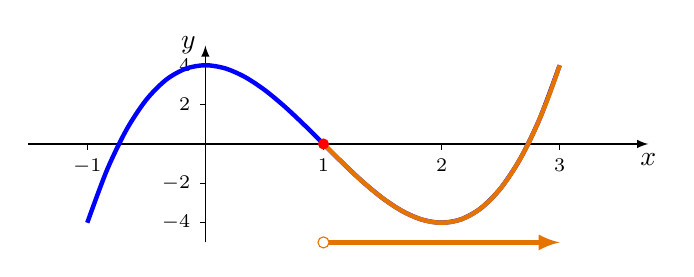
\begin{tikzpicture}[x=15mm,y=2.5mm,>=latex]
    %
    \draw[thin,black,->] (-1.5,0) -- (3.75,0) node[below] {$x$};
    \draw[thin,black,->] (0,-5) -- (0,5) node[left] {$y$};
    % ticks:
    \foreach \x in {-1,1,2,3}
    {
      \draw[thin,black] (\x,0) -- (\x,-2pt) node[below] {$\scriptstyle\x$};
    }
    \foreach \y in {-4,-2,2,4}
    {
      \draw[thin,black] (0,\y) -- (-2pt,\y) node[left] {$\scriptstyle\y$};
    }
    \draw[ultra thick,blue,domain=-1:3,smooth] plot (\x,{2*(\x)^3-6*(\x)^2+4});
    \uncover<4->{%
      \draw[ultra thick,orange!90!black,domain=1:3,smooth] plot (\x,{2*(\x)^3-6*(\x)^2+4});
      \draw[ultra thick,orange!90!black,->] (1,-5) -- (3,-5);
      \draw[orange!90!black,fill=white] (1,-5) circle (2pt);
      \fill[red] (1,0) circle (2pt);
    }
  \end{tikzpicture}
  \hfill
  \ 
  \vspace*{-1em}

  \begin{center}
    A\ when $x<2$
    \quad 
    B\ when $x>2$
    \quad
    C\ when $x<1$\\
    \ 
    \quad 
    D\ when $x>1$
    \quad
    E\ when $-0.7<x<1$
    \pause
    \quad
    \uncover<4->{\fbox{D}}
  \end{center}
}

}


\section{Max / Min Review}

\frame{
  \frametitle{\S8.13: Max/Min problems}

  Often want to find the biggest, smallest, most, least, maximum, minimum of something.

  \begin{minipage}{0.4\linewidth}
    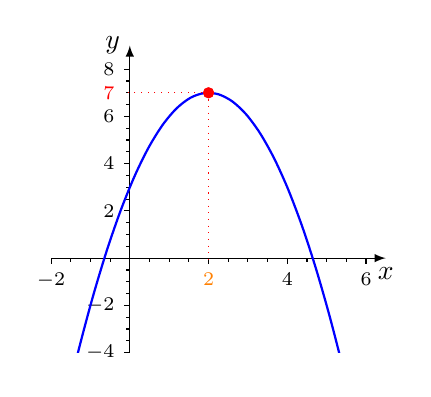
\begin{tikzpicture}[x=5mm,y=3mm,>=latex]
      \draw[thin,black,->] (-2,0) -- (6.5,0) node[below] {$x$};
      \draw[thin,black,->] (0,-4) -- (0,9) node[left] {$y$};
      % ticks:
      \foreach \x in {-2,2,4,6}
      {
        \draw[thin,black] (\x,0) -- (\x,-2pt) node[below] {$\scriptstyle\x$};
      }
      \foreach \x in {-2,-1.5,...,6.2}
      {
        \draw[thin,black] (\x,0) -- (\x,-1.5pt);
      }
      \foreach \y in {-4,-2,2,4,6,8}
      {
        \draw[thin,black] (0,\y) -- (-2pt,\y) node[left] {$\scriptstyle\y$};
      }
      \foreach \y in {-4,-3.5,...,8.2}
      {
        \draw[thin,black] (0,\y) -- (-1.5pt,\y);
      }
      \begin{scope}
        \clip (-2,-4) rectangle (6,8);
        \draw[thick,blue,domain=-2:6.5,smooth] plot (\x,{-1*(\x)^2+4*\x+3});
      \end{scope}
      \uncover<2->{%
        \draw[thin,red,dotted] (2,7) -- (-2pt,7) node[left] {$\scriptstyle7$};
        \fill[red] (2,7) circle (2pt);
      }
      \uncover<3->{%
        \draw[thin,red,dotted] (2,7) -- (2,-2pt) node[below,orange,fill=white] {$\scriptstyle2$};
        \fill[red] (2,7) circle (2pt);
      }
    \end{tikzpicture}
  \end{minipage}
  \hspace*{0.25in}
  \parbox{50mm}{%
    Here's the graph of \\
    $y = f(x)=-x^2+4x+3$
    \gap

    \uncover<2->{%
      The \emph{maximum value} or just \emph{maximum} of the function is ${\red 7}.$ 
    }
    \gap

    \uncover<3->{
      The \emph{value of $x$}\ which gives the maximum of $f(x)$ is $x={\orange 2}$
    }
    \gap

    \uncover<4->{%
      We write ${\blue f({\orange 2})} = {\red 7}$.
    }
  }
  \gap

  \uncover<5->{%
    For this example you can see this is the maximum because
    \begin{equation*}
      f(x) 
      = -x^2+4x+3
      = -(x-{\orange 2})^2+{\red 7}
    \end{equation*}
    $(x-{\orange 2})^2$ is always positive except when $x=\orange 2$\\
    {\blue so the maximum  must} be at $x=\orange 2$.
  }

}

\frame{
  \frametitle{How To Find A Max / Min}

  \begin{mdframed}[style=FactStyle]
    \begin{itemize}
    \item[{\red(1)}] Find $f{\red '}(x)$

    \item[{\red(2)}] Solve $f{\red '}(x)=0.$ This is the $x$ value
      that gives the max / min. 

    \item[{\red(3)}] To find the maximum / minimum plug the value of $x$ found
      in {\red(2)}\ back into $f(x)$. 

    \end{itemize}
  \end{mdframed}
  \vspace*{0.5in}
  \pause

  \alert{Example:}\ Use this method to find the $x$-value where
  \emph{maximum}\ of the function $f(x)=5x-e^{2x}$ occurs.
  \begin{center}
    A $=0$
    \quad 
    B $= \ln(5)$
    \quad 
    C $= 2\ln(5)$
    \quad 
    D $= 2\ln(5/2)$
    \quad 
    E $= \ln(5/2)/2$
    \pause
  \end{center}
  \alert{Answer:}\ \answer{E}
  \vspace*{1in}


}


\section*{Review problems}

\frame{
  \frametitle{Word Problem \#8}
  
  A farmer is growing wheat.
  \begin{itemize}
  \item On July 1, she has $1,000$ bushels and this increases by $50$
    bushels per day. 

  \item The price of a bushel on July 1 is $\$10$ and is dropping at a rate of $20$ cents per day. 

  \item She will harvest and sell on the same day. 
  \end{itemize}
  How many days should she wait, assuming these trends continue?
  \begin{center}
    A $= 5$
    \quad 
    B $= 10$
    \quad 
    C $= 15$
    \quad 
    D $= 20$
    \quad 
    E $= \text{other}$
    \pause
    \quad
    \fbox{C}
  \end{center}
  \vspace*{2in}

}


\frame{

\centerline{\Huge \blue Some Review Problems} \vspace{20pt} 

\centerline{\Huge \blue From Webwork}

\begin{center}
{\red {\bf *} An old midterm may be reviewed in class instead.

This midterm will be posted with worked out solutions.}
\end{center}

}


\frame{
\frametitle{Unit Conversion Problem}
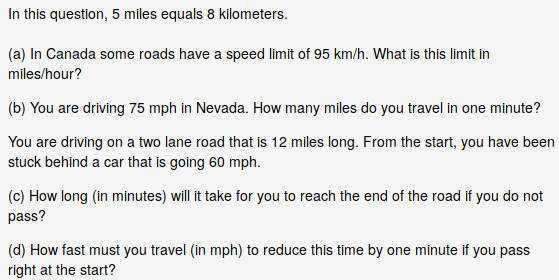
\includegraphics[scale=0.6]{HW03.png}
}

\frame{
\frametitle{Line Equation Problem}
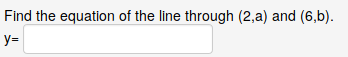
\includegraphics[scale=0.7]{HW04.png}
}


\frame{
\frametitle{Linear Modeling Problem}
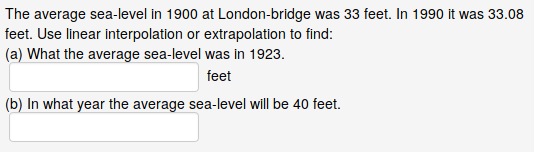
\includegraphics[scale=0.6]{HW05.png}
}


\frame{
\frametitle{Average Rate of Change Problem}
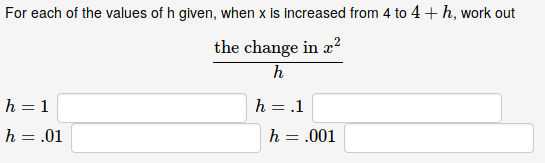
\includegraphics[scale=0.6]{HW06.png}
}

\frame{
\frametitle{Log Properties Problem}
\begin{itemize}
\item\pause
Rewrite $\log(xy)$.
\item\pause
Rewrite $\log(x+y)$.
\item\pause
Rewrite $\log(x-y)$.
\item\pause
Rewrite $\log(x)-\log(y)$.
\item\pause
Rewrite $\log(1/\sqrt{x})$.
\end{itemize}
}

\frame{
\frametitle{Percent Word Problem}
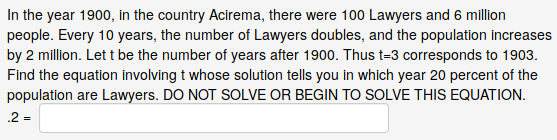
\includegraphics[scale=0.6]{HW09.png}
}

\frame{
\frametitle{Speed Estimation Problem}
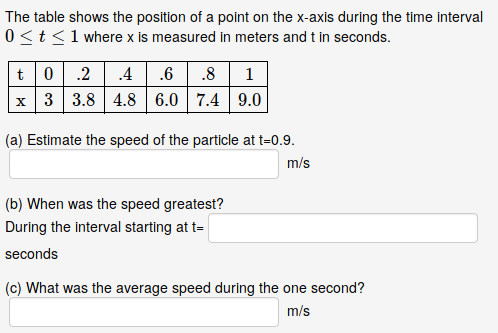
\includegraphics[scale=0.6]{HW10.png}
}


\frame{
\frametitle{Exponential Decay Problem}
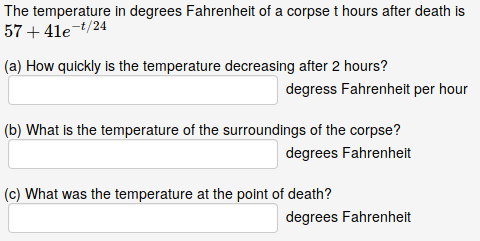
\includegraphics[scale=0.6]{HW14.png}
}

\frame{
\vfill
{\large \blue Please fill out evaluations for the course.
\\
Your feedback is helpful!} 
\vfill
}




\end{document}


